
%(BEGIN_QUESTION)
% Copyright 2006, Tony R. Kuphaldt, released under the Creative Commons Attribution License (v 1.0)
% This means you may do almost anything with this work of mine, so long as you give me proper credit

Grunnligningen for en orifiseplate bygger på Bernoullis lov:

$$z_1 \rho g + {v_1^2 \rho \over 2} + P_1 = z_2 \rho g + {v_2^2 \rho \over 2} + P_2$$

$$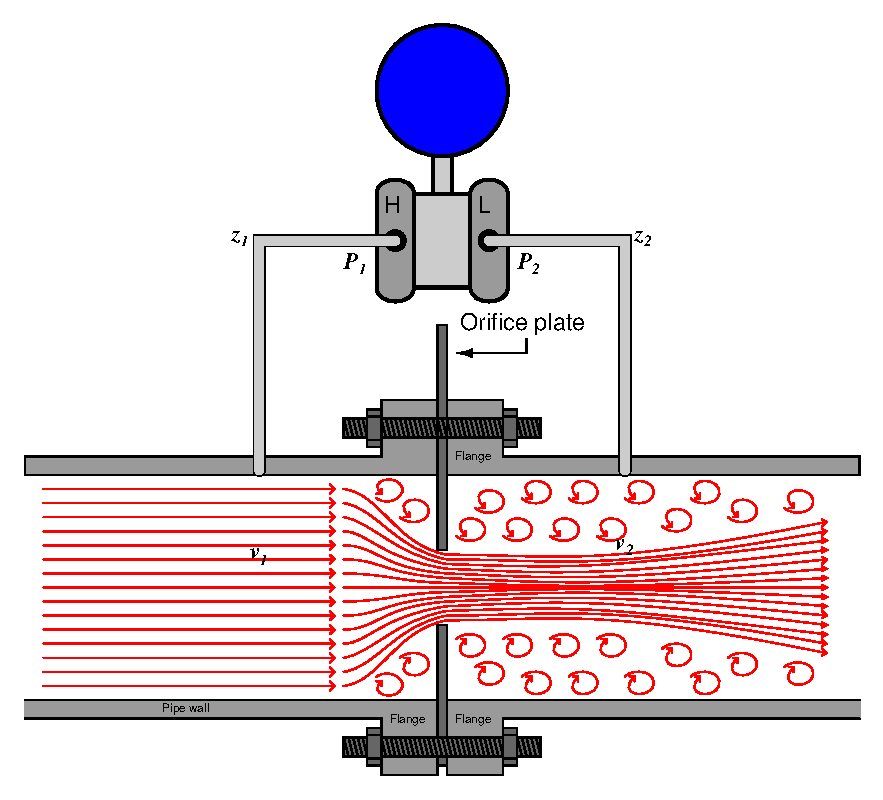
\includegraphics[width=15.5cm]{i00731x01.eps}$$

Med lik høyde i målepunktene $z_1$ og $z_2$ forenkles ligningen:

$${v_1^2 \rho \over 2} + P_1 = {v_2^2 \rho \over 2} + P_2$$

Samle ledd:

$$P_1 - P_2 = {v_2^2 \rho \over 2} - {v_1^2 \rho \over 2}$$

$$\Delta P = {\rho \over 2}({v_2^2 - v_1^2})$$

$${{2 \Delta P} \over \rho} = {v_2^2 - v_1^2}$$

Hvis hastigheten i vena contracta er betydelig større enn hastigheten i fullt rør, kan vi approksimere:

$${{2 \Delta P} \over \rho} \approx v_2^2$$

$$v_2 \approx \sqrt{{2 \Delta P} \over \rho}$$

Siden $v_2$ relaterer direkte til strømning ($Q$), kan vi skrive:

$$Q = k \sqrt{{\Delta P} \over \rho}$$

Basert på denne ligningen: hva gjør en differansetrykktransmitter hvis fluidet gjennom orifiseplaten plutselig blir {\it tettere}, uten endring i volumstrøm (dvs. samme rørhastighet $v$, men høyere $\rho$)?

\underbar{file i00731}
%(END_QUESTION)





%(BEGIN_ANSWER)

Hvis $\rho$ øker uten endring i $v$, vil differansetrykket $\Delta P$ øke.

\vskip 10pt

Hvis $\rho$ dobles, dobles også $\Delta P$. Men for å representere en dobling i flow måtte $\Delta P$ økt med faktor {\it fire (4)}, siden $\Delta P$ normalt kvadratrotslineariseres. En dobling av tetthet gir derfor indikert flowøkning med faktor $\sqrt{2}$.

%(END_ANSWER)





%(BEGIN_NOTES)


%INDEX% Måling, flow: orifiseplate

%(END_NOTES)
